% THIS IS SIGPROC-SP.TEX - VERSION 3.1
% WORKS WITH V3.2SP OF ACM_PROC_ARTICLE-SP.CLS
% APRIL 2009
%
% It is an example file showing how to use the 'acm_proc_article-sp.cls' V3.2SP
% LaTeX2e document class file for Conference Proceedings submissions.

\documentclass{acm_proc_article-sp}

\begin{document}

\title{uF!t: A Framework for Monitoring Exercises}

% \subtitle{[Extended Abstract]
% \titlenote{A full version of this paper is available as
% \textit{Author's Guide to Preparing ACM SIG Proceedings Using
% \LaTeX$2_\epsilon$\ and BibTeX} at
% \texttt{www.acm.org/eaddress.htm}}}

%
% You need the command \numberofauthors to handle the 'placement
% and alignment' of the authors beneath the title.
%
% For aesthetic reasons, we recommend 'three authors at a time'
% i.e. three 'name/affiliation blocks' be placed beneath the title.
%
% NOTE: You are NOT restricted in how many 'rows' of
% "name/affiliations" may appear. We just ask that you restrict
% the number of 'columns' to three.
%
% Because of the available 'opening page real-estate'
% we ask you to refrain from putting more than six authors
% (two rows with three columns) beneath the article title.
% More than six makes the first-page appear very cluttered indeed.
%
% Use the \alignauthor commands to handle the names
% and affiliations for an 'aesthetic maximum' of six authors.
% Add names, affiliations, addresses for
% the seventh etc. author(s) as the argument for the
% \additionalauthors command.
% These 'additional authors' will be output/set for you
% without further effort on your part as the last section in
% the body of your article BEFORE References or any Appendices.

\numberofauthors{2}

%\author{
% You can go ahead and credit any number of authors here,
% e.g. one 'row of three' or two rows (consisting of one row of three
% and a second row of one, two or three).
%
% The command \alignauthor (no curly braces needed) should
% precede each author name, affiliation/snail-mail address and
% e-mail address. Additionally, tag each line of
% affiliation/address with \affaddr, and tag the
% e-mail address with \email.
%
% 1st. author
% \alignauthor
% Ben Trovato\titlenote{Dr.~Trovato insisted his name be first.}\\
%        \affaddr{Institute for Clarity in Documentation}\\
%        \affaddr{1932 Wallamaloo Lane}\\
%        \affaddr{Wallamaloo, New Zealand}\\
%        \email{trovato@corporation.com}
% % 2nd. author
% \alignauth`or
% G.K.M. Tobin\titlenote{The secretary disavows
% any knowledge of this author's actions.}\\
%        \affaddr{Institute for Clarity in Documentation}\\
%        \affaddr{P.O. Box 1212}\\
%        \affaddr{Dublin, Ohio 43017-6221}\\
%        \email{webmaster@marysville-ohio.com}
% }

\author{
\alignauthor
Brandon Snuggs\\
       \affaddr{Swarthmore College}\\
       \affaddr{500 College Avenue}\\
       \affaddr{Swarthmore, Pennslyvania}\\
       \email{bsnuggs1@swarthmore.edu}
% 2nd. author
\alignauthor
Steven Hwang\\
       \affaddr{Swarthmore College}\\
       \affaddr{500 College Avenue}\\
       \affaddr{Swarthmore, Pennslyvania}\\
       \email{shwang1@swarthmore.edu}
}

\maketitle
\begin{abstract}
Common reasons for the low motivation to exercise include
the absence of an exercise partner and the large time investment
required in traveling to the gym. Some responses to this
issue have divulged possible solutions: joining an exercise
support groups or focusing on exercises that can be done without
gym equipment. While both suggestions are practical, 
studies show support groups are notable in that they have 
been known to be effective at keeping individuals adhere to a
regular exercise routine. Furthermore, the modern evolution of
social networking sites has allowed for support groups to form
online.

It should be noted that there are a multitude of engaging
exercises that can be done with minimal gym equipment 
(i.e. pushups, situps, yoga); however, it is often a hassle to
mentally keep track of all these exercises. We present uF!T, as
a framework that leverages the benefits of exercise support
groups and provides tools to monitor and count exercises done
inside and outside the gym. uF!T attempts to take advantage 
of static position measurement accuracy in an accelerometer
and the smoothness of gyrometer measurements in a complementary
filter to reduce noisy measurements. Our evaluation of uF!t
includes experiments on proper sensor placement and will 
include tests on classification accuracy.
\end{abstract}

\section{Introduction}
Currently, America's healthcare costs have been rising more 
and more each year. One of the most influencing factors in this
phenomenal increase is due to obesity. In 2008, obesity healthcare
costs account for at least 10 of total medical expenditures \cite{jeffords:obesity}.
This amounts to 147 million dollars a year. Currently, in addition to
experiencing trouble with sticking to drug regiments, doctors also have
trouble making their patients still to their exercise schedule.  In a
case study involving 20 patients, on the first day all patients agreed
that they would stick to their regiment, but after three months, only
seven patients were still doing their exercise regiment.  In eight months,
only five were still doing their regiment \cite{campbell:noncompliance}. This is
the same for regular citizens joining exercise programs in America.  Current
studies show that 50\% of Americans that join an exercise program, will drop
out within the first six months \cite{kravitz:eMotivation}.

\begin{figure}
\centering
\includegraphics[width=3.0in,width=3in]{./figs/dontexercise.png}
\caption{Some of the many reasons for not exercising.}
\label{fig:noexercise}
\end{figure}

\subsection{Why don't people exercise?}
While exercise is the main solution to help reducing obesity, people still
choose to not exercise despite the health benefits that it imposes.  Some
researchers believe that this is due to the increase in fast-paced lifestyles.
In many cases, people just simply state that they do not have the time to stick
to an exercise schedule, either due to long work hours or other schedules (\textit{picking
up kids, attending city meetings, taking care of family, etc.}) that
makes people generally unavailable.

Researchers claim that the general decrease in exercise in
the US population is is mainly a consequence of technology
replacing usual forms of exercising. Earlier in America history, traversing long
distances were completed by either walking or riding a bicycle, whereas now such 
distances are covered by either driving or use of public transportation
(which generally involve an individual to be sitting). As technology has advanced,
more and more activites that required physical activity are now being phased out.  Even
the household vaccuuming can be replaced by purchasing a Roomba robot.
In addition to fast-paced lifestyles and unavailable schedules, researchers attribute
people's lack of motivation to workout to several different reasons as seen in figure
\ref{fig:noexercise} . Looking at the figure, we can see that lack of motivation is 
due to inability to obtain moral support from apartner or support group.  
It has been proven that people are more inclined to stick to an exercise regiment
if they have a friend or family member that can assist them \cite{plante:exercisewithanother}.
By merely having an exercise partner, it improves the amount of stress relieved
during a regular exercise routine.  Admittedly, we do not believe that uF!t is capable
of solving every problem listed in the figure.  However, we believe that uF!t has the
possibility to solve two problems: \textit{no exercise partner} and \textit{lack of time}.

\section{SYSTEM ARCHITECTURE}
Our system will consist of the following components: Workout 
classifier, exercise counter, wireless data transfer protocol 
and Social Media application.

\subsection{Workout classifier}
uF!T will interpret accelerometer and gryoscope data in order
to determine what exercise is being performed. Our current 
classifier will distinguish exercises according to sensor 
measurement values along the x, y and z axes. Sensors measure-
ments would include rotational velocity around each axis and 
acceleration along each axis and be stored in a 6-tuple. The
k-means classification algorithm would be used to group sets 
of sensor measurements into clusters where we assume each 
cluster would represent an exercise.

Therefore, successive measurements that obtain values that are
similar in value to a cluster would be grouped with it. 
Practically, the classifier would consider a fixed number 
(100 samples) of sensor measurements at a time.

The following describes the k-means algorithm:

\begin{enumerate}
\item Place K points into the space represented by the objects that are being clustered. These points represent initial group centroids.
\item Assign each object to the group that has the closest centroid.
\item When all objects have been assigned, recalculate the positions of the K centroids.
\item Repeat Steps 2 and 3 until the centroids no longer move. This produces a separation of the objects into groups from which the metric to be minimized can be calculated.
\end{enumerate}

After clusters are determined, we would classify incoming data
according to which cluster center they most resemble. We note
that we have not classified the characteristics of many exercises
besides a situp. Furthermore, it is possible to have an individual
do an exercise that is currently not defined. In this case, this
exercise would be classified as an unknown exercise and still be
tracked and counted. For practical purposes it is likely for some
exercises to not be defined given the limited space on the mote 
that is available to store exercise classification information.
Nevertheless, the user would be given the option of specifying a
name for this exercise so that it could be tracked in the future.

\subsection{Exercise Counter}
After an exercise has been classified, we would begin counting 
noticable features of the exercises in order to keep track of the number 
of repetitions that have been completed. For example, in our current
iteration we have completed the situp detector.  When a user is doing
a situp, their body oscillates between two varying angles: the rest
and the peak.  We currently can count the amount of rest-peak pairs that
have been completed, thus representing the amount of situps completed.
We believe we can use this same strategy to detect other exercises, such
as push-ups, which also have a similar oscillation, but it is represented
vertically and not angular like a situp.  With exercises having this similar
repeated motion, we believe that we will be able to count a wide range of
calisthenics.

\subsection{Peak detection}
In order to recognize a peak in the measurement data, such as the angles
found from our situp detector, we would like to set threshold values that
would represent the minimum value to be considered a rest
and the maximum value to be considered a peak.  Each peak in the measurement
readings would consist of data points that are above the peak 
threshold value. It is common to have multiple data points 
classify to be a peak value. The number of successive peak values
indicate confidence that a peak is correctly observed. Typically,
higher frequencies in a given would indicate a stronger confidence
that a peak is indeed there while lower frequencies (one or two 
peak detections) might indicate some noise. In order to make our 
system more robust to misclassification due to noise we propose 
the following conditions:

\begin{enumerate}
\item In order to be classified as a peak there must be at least 3 consecutive peak classifications. Otherwise, the classification is assumed to be from noise.
\item If a peak is classified recently another peak classification would be counted toward the recent peak instead of classifying a new peak.
\end{enumerate}

Furthermore, threshold values are initially chosen by hand. 
In order to account for the potential to have different forms of 
data for individuals, these threshold values will be user-specific.
We hope to gain this information by dynamically updating these 
threshold values and store these in a user profile on the social
media application.

\subsection{Wireless Protocol}
The motes will communicate with a base station based on a passive
architecture. Passive communication architecture has shown to 
reduce the usage of the motes radio for needless transmissions.
According to this architecture, a base station will constantly be
transmitting queries for information. Once a mote is within range
of a base station, the mote will attempt to establish stable 
connection and transmit the user's exercise information.

The wireless protocol of this framework would also implement 
synchronous communication that would reduce the amount of time 
needed to listen for a response [13].

Both features of the protocol are will increase the lifespan of
the mote's battery. In order to reduce extraneous use of radio given
that the use of radio has been known to be a component that would
drain a mote's battery the most rapidly.

\begin{figure}
\centering
\includegraphics[width=2.0in,width=2in]{./figs/situpsfbtwit.png}
\caption{The current casing for our uF!t device.}
\end{figure}


\subsection{Social Media Application}
Our framework plans to have a base station connect to a server for
storage of user profiles. Users would be able to login into a Facebook
application in order to view and share their exercise history with 
friends. A primary feature of the Facebook application would be the 
game component of the application. Users would rewarded for completing
exercise goals and in turn use their rewards to their advantage in an
online game. The game would involve a system where cumulative progress
is visible (i.e. building a fortress with upgraded turrets to defend 
against barbarian hordes). Furthermore, the Facebook application would
also serve to store user-specific information that would allow for 
dynamic exercise classification. Each user would have associated 
threshold values for each exercise they regularly complete. It is 
possible for these threshold values to be updated regularly (i.e. if
the user improves their form when engaging in exercises or if default
threshold values are too high or too low). Therefore, each time the base
station communicates with the mote and receives feedback on improving the
threshold values, the Facebook application would store these new threshold
values. 
\begin{figure}
\centering
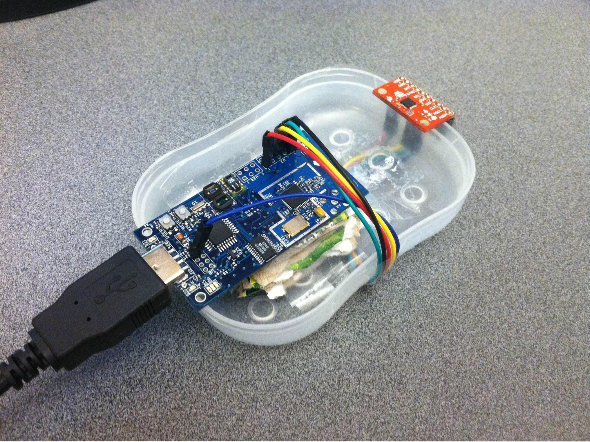
\includegraphics[width=2.0in,width=2in]{./figs/tmotesky.png}
\caption{The current casing for our uF!t device.}
\label{fig:devicecase}
\end{figure}

\section{Implementation}
We used the Tmote Sky for the basis of our project. The Tmote 
Sky can be powered by two AA batteries, however in our current 
implementation of uF!t, it is still wired, thus not requiring the use
of batteries.  Besides the electrical components, we have encased our
device using a lightweight plastic container (similar to a soap bar case).
The housing for our device helps the sensor sit in a stable position.
The data is already noisy, so it is important that the sensors are not
given more opportunities to be mutated by noises induced by the sensor
rocking carelessly.

\subsection{Software: Contiki 2.6}
Unlike a standard out-of-the-box Tmote Sky, we use Contiki 2.6, instead of
using TinyOs.  We chose to make this decision since our team was much
more familiar with C, which made it much easy for us to quickly
understand native functions in Contiki 2.6.  Additionally, this allowed
us to focus on understanding how to integrate the accelerometer and
gyroscope's functionality into Contiki.

\subsection{Hardware: mpu6050}
We have connected the 3-axis Gyro/Accelerometer mpu6050.  The gyroscope
contains various degrees of sensitivity, which can be easily
modified with Contiki functions that we have created. The mpu6050 sensor
also contained a temperature gauge; for the time being, we did not 
incorporate the temperature gauge into our project, but we believe it may
have later uses (for more info please look at future works).

To ensure that we could track a user's body while doing a situp,
this required more work than just using the accelerometer and 
gyroscope raw data to do localization.  As such, we ran through
some equations that either used the accelerometer or the gyroscope.
However, after running some tests seperately on the accelerometer and
gyrscope, we decided that we would need to use the measurements received
from both devices in order to calculate the angle of user's body.

\subsection{Accelerometer}
In order to track simple movements like a push-up or sit-up,
it was easy to determine by focusing on variation in the 
accelerometer's z (for the push-up) and the accelerometer's
y (for a pull-up).  However, in order to calculate the angle
of the user's body with respect to our sensor, requires some
trigonometry.

\begin{equation}angle_{accel_x} = \arctan(accel_x,accel_z) + \pi\end{equation}

Using the equation above allows us to calculate the tilt angle 
for the accelerometer.  Remember that arctan, known as atan2
in contiki, outputs between the range of \(-\pi\) and \(\pi\), so you
must add \(\pi\) to the results of arctan to have the range convert-
ed to 0 to 2\(\pi\).  Having no initial knowledge in the usage
of accelerometers or gyroscopes, we believed that the accelero-
meter would have served its purpose for calculating the wearer's
body angle during a situp.  However, if we look at figure \ref{fig:accelResults}
we can see that our initial assumption was clearly untrue.  The
accelerometer is great at calculating angles for stationary 
positions, but it is terrible at tracking the rapid movements 
experienced during a situp.  After doing a realtime comparison
of an actual situp and the data we recorded, it turns out that
the accelerometer reports angles exceedingly lower than what is
actually completed.  In our initial tests, we only did situps
up to angle of \(60^\circ\), however when we look at figure \ref{fig:accelResults},
we can see that the highest recorded peak is about \(40^\circ\).  Additionaly,
the data that we received was noisy, so this was unsuitable for
accurately tracking a user's angle.

\begin{figure}
\centering
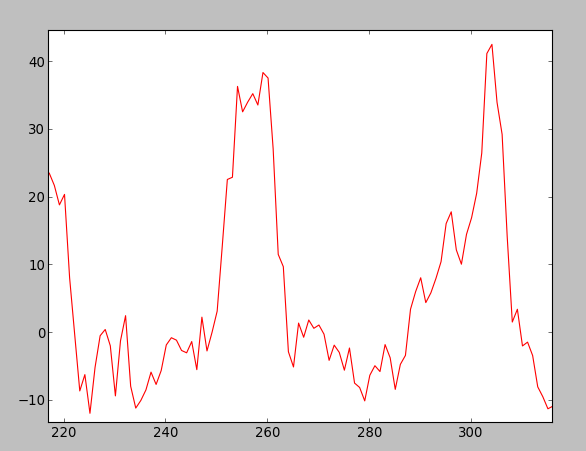
\includegraphics[width=3.0in,width=3in]{./figs/accel_test.png}
\caption{The results of the accelerometer.}
\label{fig:accelResults}
\end{figure}

\subsection{Gyroscope}
The gyroscope is able to calculate angular velocity in degrees 
per second, which lead us to think that the gyroscope would
provide more promising results.  For the gyroscope, we used 
this simple equation to calculate the angle.

\begin{equation}angle_{gyro_x} = angle_{gyro_x} + gyro_x*dt\end{equation}

Gyro is the degrees per second (\(^\circ/s\)) recorded from the
gyroscope, while delta t is the sample period calculated from 
the sample speed.  
Multiplying the gyro by sample period, gives us the angle calculated 
within one cycle, which can be accumulated in our total angle.  
Successfully being able to calculate the angle using the gyro, 
we were certain that our results would be promising.  Looking
at figure \ref{fig:gyroResults}, however, the gyroscope's measurments are 
constantly increasing by a fixed amount as time goes on, this
is called \textit{drift}.  From our gryoscope analysis, the
gyro not only experiences drift (about \(5^\circ/s\)),
but it also is not centered properly.  Currently, when the gyroscope is
stationary, it returns an angular velocity of \(34^\circ/s\).
in motion.

\begin{figure}
\centering
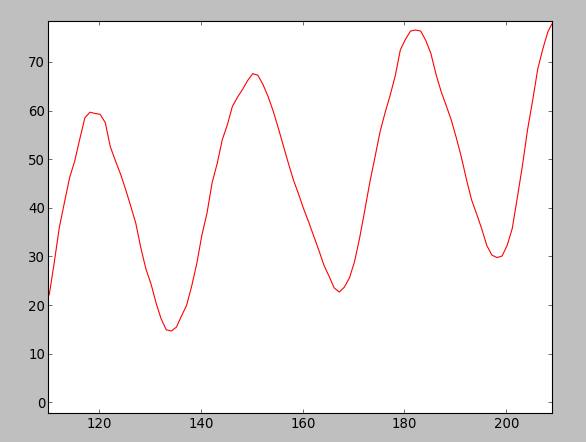
\includegraphics[width=3.0in,width=3in]{./figs/gyro_test.png}
\caption{The results of the gyroscope, smoother than the
accelerometer results.}
\label{fig:gyroResults}
\end{figure}


\subsection{Complimentary Filter}
From our analysis, we can see that both accelerometers and 
gyroscopes have their own pros and cons.  The accelerometer 
is really good at detecting static positions, however whenever
it is moving very quickly, it returns very noisy data.  In 
contrast, the gyroscope is really good at detecting rapid 
movements, however its data drifts over time, making it 
increasingly inaccurate the longer you monitor the gyroscope.
This lead us to using the complimentary filter.

\begin{equation}angle_x = (a)*(angle_x+gyro_x*dt)+(1-a)*(angle_{accel_x})\end{equation}

With the knowledge that we cannot rely on the gyroscope for 
long periods of time, it is important to calculate a good time
constant.  The time constant helps determine the coefficients 
used in the filter.

\begin{equation}\tau = \frac{a*dt}{1-a}\end{equation}

The time constant may vary from user to user depending on
the reliability of the gyroscope's data and the sample
rate.  The time constant defines the boundary between
trusting the gyroscope and trusting the accelerometer.
In our time constant, we used a time constant of \textit{.5
seconds}. We had chose this time constant due to our results
from the gyroscope.  It is important to choose a time constant
that will work with the amount of drift generated from the
gyroscope.  This means that for any measurement that is
lower than half a second, the algorithm will take the
gyroscope's measurements into consideration.  However,
for any measurements that take longer than half a second,
the accelerometer will have more weight, allowing it to
take precedence over the gyroscope.  Remembering that
the gyroscope drifts over time, so for the results that
are recorded short periods, such as a quick rise during
a situp, it is very reliable.  However, consider a user
that has already risen and is waiting at the peak of their
situp.  In this situation, the gyroscope will become
unreliable as time continues to expire, so it is better
to trust the accelerometer's data because it is suited
for recording angles in stationary positions.  Using the
complementary filter in this style, allows us believe that
we will be able to record situps at varying speeds.


\section{Evaluation}
In order to estimate how well our uF!t system is working, it
will require the evaluation of two things: Peak Detection
and Proper Sensor Placement.  Peak Detection allows us to
determine whether the user has successfully completed a situp
or not.  This algorithm is important in being able to correctly
detect a situp.  Without good recognition of a simple situp,
we would be unable to trust our system, which means that we
would not able to further implement new exercises on our system.
Proper Sensor Placement is important for making sure that
the data we record is consistent.  By placing uFit in neg-
lible areas, the data may suffer from additional unwanted 
noise, which would make it more difficult to detect good
exercises.

\subsection{Peak Detection}
There are two important terms that we use for our Peak
Detection algorithm: \textit{peaks} and \textit{rests}.
Peaks are moments where the user has effectively slowed
their angular velocity to 0, while also being above a
threshold value.  Rests are the complete opposite, they
are moments where the user's angular velocity is close to 0,
while also being below a threshold value  In our current 
implementation, we have designated zones to represent "good"
areas for peaks and "good" areas for rests.  These "good" areas
are set by threshold values that has been determined by us
for our studies. \(50^\circ\) or higher represents the
threshold value for peaks, while \(10^\circ\) or below
represents the threshold value for rests.  We have chosen
these threshold values based upon monitoring other people who
were doing situps. Of course, we admit that currently having
static threshold values is not the best implementation for
detecting situps.  However, we found threshold values provided
us a quick and simple way to begin detecting situps without
having to use anything that is computationally heavier.  Looking
at Figures \ref{fig:centerchest}, \ref{fig:sidechest}, and \ref{fig:sidearm}, 
we already have results from the threshold values that we selected.
The upper blue dots, represents detected peaks, while the lower green
dots represent detected rests. Like our competitors, we too have provided
in-sensor calculations, allowing us to minimize the amount of data that
will be sent once we begin working on wireless communication support.


\begin{figure}[!ht]
\centering
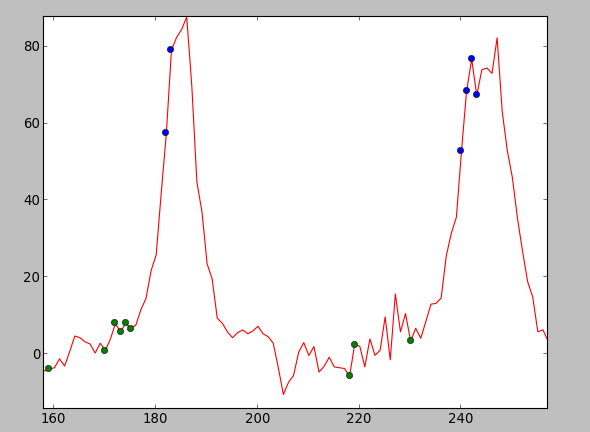
\includegraphics[width=3.0in,width=3in]{./figs/chestTestcenter.png}
\caption{The results of the complimentary filter with sensor placed
on the center of the chest.}
\label{fig:centerchest}
\end{figure}

\begin{figure}[!ht]
\centering
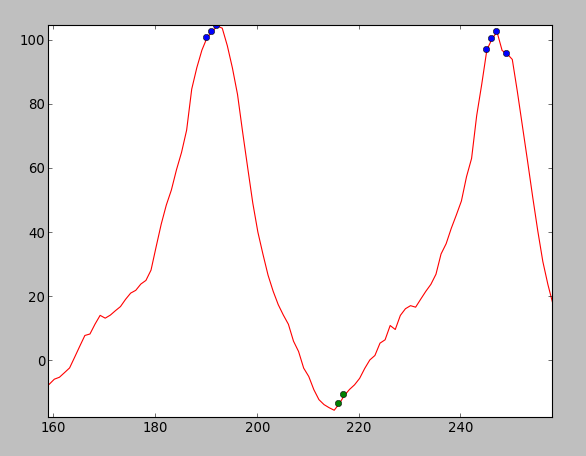
\includegraphics[width=3.0in,width=3in]{./figs/chestTestside.png}
\caption{The results of the complimentary filter with sensor placed
on the side of the chest.}
\label{fig:sidechest}
\end{figure}

\subsection{Proper Sensor Placement}
For testing proper sensor placement, we tested several
areas where the sensor could be placed on a user's body.
As stated earlier, it is important to choose a good location for the 
system since it may affect the overall quality of the data.  Additionally, we must consider whether
or not if the placement of the sensor is comfortable for
the user.  In our prelimenary tests, it seems that it was
acceptable to place the device on the following three
places: \textit{the arm, center of chest, and the side 
of the chest.} We assumed that the center of the chest
would provide us with the most accurate data, since it
is centered at the body and it should not affect any of
the data since the chest area is generally an even area
for people of most sizes.

Looking at the graphs depicted in Figures \ref{fig:centerchest}, \ref{fig:sidechest}, and \ref{fig:sidearm} , we see that
our initial assumption was actually incorrect.  It seems
that the sensor obtained the best results when it was
placed on the side of the chest.  Of course, we expected
that the arm would not be the best place since depending
on the user, they may either do a situp with their arms
placed on the side of their body, or they may do it with
their arms crossed across their chest.

These results were nice for our initial attempts, however,
we believe that it lacks the diversity of different sized
bodies for the test results.  We believe that if we can
get more people for our analysis, we can see if the positions
that we have provided are universally good for different
sized people.  So far our preliminary results have been
tested on average-sized males, which currently is a limited
scope of view considering that we wish this device to be
used by many people.

\begin{figure}[!ht]
\centering
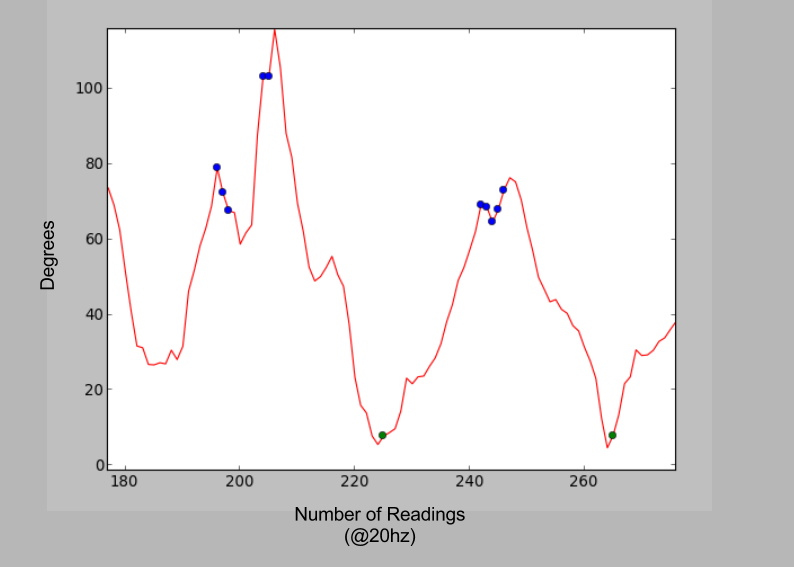
\includegraphics[width=3.0in,width=3in]{./figs/armTest.png}
\caption{The results of the complimentary filter with sensor placed
on the arm.}
\label{fig:sidearm}
\end{figure}

\subsection{Accuracy}
Remembering the last section, we determined that it
is important that we are able to detect the correct amount
situps with indivudals of varying body types.  For our next
tests, we used four random individuals to do situps while
wearing our uF!t device.  Each user was properly informed
about what our device is capable of, and they were given the
choice to decline if neccessary.  Our test comprised of
three different situp speeds: \textit{fast, normal,} and
\textit{slow}.  Fast is equivalent to completing a situp every
second, while normal is completing a situp every two seconds
and slow is completing a situp every three seconds.  The
objective of each testing speed was to complete ten situps.

To ensure that each set of situps was completed in the same
fashion, participants were given a 10 minute break to allow
them to recouperate if they were feeling fatigued.  Determing
the accuracy of each setup involving the comparison between
the amount of situps that uF!t detected and the amount situps
counted.  As stated earlier, the stress of workout can impact
a person's ability to record situps.  To avoid the human error
of our participants, we allowed third parties to count the
amount of situps being done for each subject.

For our sampling speed, we chose 20hz for our measurements.  As seen in some related
works, there have been tests using higher sampling speeds to
record data \cite{farringdon:sensorbadge}.  However, when reading
about the SATIRE device, their group was able to achieve decent
readings with using only 25hz \cite{ganti:satire}.  In accordance with our
future works for uF!t, we wish our device to be usable on the go.
We will not be able to accomplish this goal if our device consumes
too much energy. Higher sampling speeds means that our device will
have higher power consumption.  In our initial design of uF!t,
we found that 20hz was the lowest sampling speed possible while
still producing reasonable results; lower sampling speeds were unable 
to keep up with the slowest situp speed.



If we look at the table 1, it seems that our device is highly accurate
when the user is utilizing a slow situp speed (average of .8).  Unfortunately,
as the user completes sit-ups at a normal speed, the device's accuracy
drops by a factor of 1.88 (average of .425).  This accuracy drops even
further when the user is completing situps at a fast speed, dropping
by a factor of 5.3 when compared to the slow situp speed.  



\subsubsection{Participant's Comments}
Considering that we intend uF!t to be used by different people, it is
important to record our participants initial thoughts about our device.
After the completion of the test, each participant was allowed to see
the results of their situps and were asked a small questionaire with the
following questions:

\begin{table*}[!htp]
\centering
\caption{Accuracy of Situps}
\begin{tabular}{|c|c|c|c|} \hline
Participants&Accuracy (Slow)&Accuracy(Normal) & Accuracy(Fast)\\ \hline
1 & .8 & .4 & .2\\ \hline
2 & .9 & .7 & .1\\ \hline
3 & .5 & .1 & .1\\ \hline
4 & .8 & .5 & .2\\ \hline
Average & .8 & .425 & .15 \\ \hline
\end{tabular}
\end{table*}

\begin{enumerate}
\item Do you consider yourself a casual or hardcore exerciser?
\item Did you like using the uF!t device? Was it comfortable?
\item Any additional comments?
\end{enumerate}

Out of the four test subjects, two identified
theirselves as casual exercises saying that they enjoyed that the
device was able to track their situps when they were completing a
slow set.  However, the other two participants that classified as 
hardcore did not appreciate that the device was unable to detect
a fast set of situps.  The hardcore exercises said that they needed
to do a larger quantity of faster situps to reap any benefits.
Some participants commented that the important part of
recording the situp is the rise.  This confirms some of our observations
during the tests where a participant's situp would not be detected until
a proper rest-peak pair was confirmed on the situp device. There were also
comments about the device still being comfortable, despite it being
worn by participants of vary sizes.  As we described in Proper Sensor Placement,
it is important to gauge the comfortability of doing the situps with the device,
since its placement can provide unneccessary noise into our data sets.


\section{Related Works}
Unlike uF!t's use of the accelerometer and gyroscope, one of our
main competitors rely on the raw measurements received from using only 3-axis accelerometers 
\cite{seeger:healthass} .  However, unlike
our design, they use multiple accelerometers.  This allows their
system to have more versatility than the amount of exercises that
we are attempting to track.  So far, our exercises are limited to
calisthenics, whereas myHealthAssistant can do resistance and 
weight training exercises.  The ability to do more of these
exercises come at a cost.  In their paper they do not cover the
amount of power consumed by using multiple sensors.  This can
make or break the effectiveness of myHealthAssistant
since it is not useful to record multiple exercises with only
a short amount of battery life.  In our current design, we admit
that we have not provided results for uF!t's battery life, too.  However,
we have not reached the phase where we can focus on analyzing
uF!t's battery life.  For these reasons, we make note of myHealthAssistant's
lack of battery life discussion because it is important reminder for a device
that is marketed to be used by people that are on the go.

SATIRE is another system that rivals some of the functionalities
that uF!t provides. In SATIRE, they create a body sensor network that is
integrated into a simple winter coat \cite{ganti:satire}.  Their work is related to
uF!t since the system they create involves determing the activity
being performed by the wearer.  They use simple actions such as
walking, sitting, climbing stairs, typing, and reading.  To monitor
these actions they use an \textit{exponential weighted moving average}
(EWMA) filter.  We find this paper very
interesting, since they use it as a way to figure out basic repetitive
actions (they provide 4 labels: stillness, typing, walking, fall).  With
the uF!t device, instead of monitoring day to day activities like SATIRE,
we wish to focus on calisthenic exercises.  Even though SATIRE is only 
for tracking normal activities, it allows them to maintain records on
the wearer's health.  uF!t provides flexibility, considering that it is
not only good for maintaining the user's health, but useful for improving
one's health as well.  Our uF!t device, once fully completed, can be
used for people and patients who wish to be healthier through doing
simple calisthenics.  As stated before, uF!t will be able to track
your progress by storing results from daily workouts, whereas SATIRE
is not neccesarily an exercise device, but only a device that
monitors your current health and activity.

Many mobile application developers have sought to provide creative solutions that complement 
a packed schedule and low interest in exercising. Mobile 
devices such as smartphones, ipods, and chips built-in shoes now
are equipped with considerable computational power and are very
portable. Some notable examples of mobile devices are as follows: Nike fit (an ipod 
application that is available on most ipod devices) is available
on many Ipod devices as an application that encourages users to
run by logging the distance run, calories burned and time of an
individual's runs. Another application is Zombierun which has 
sought to encourage individuals to exercise by introduce a gaming
aspect to the routine as well as the ability to share results via
social media. The Zombierun application has shown to be successful
by popular account and has therefore involved encouraged many people
to exercise more. Unfortunately, the Zombierun application is extremely
limited in its variety exercises.  Currently, Zombierun is only capable
of encouraging a user to run.  UF!t offers a vareity exercises, so that
a user will not have to stick to the same routine.  Being able to change
your routine has been proven to provide better health benefits, than
a routine that is always the same.

\section{Future Works}
In our current design of uF!t, we unfortunately are unable to
communicate wirelessly.  We chose this option, so that we could
focus on getting accurate results from our accelerometer and gyrscope.
However, we believe that wireless communication is the next important
step in the design of our system.  With the addition of wireless
support, it will provide the groundwork so that we can start Social media 
integration.

As stated earlier, the mpu6050 contains a temperature sensor.  In
future designs of uF!t, we believe that we can incorporate the
temperature sensor to monitor the amount of heat being generated
during a workout session.  With this data, we want to be able
to determine if the user has been working out for too long.  This
would be idealistic for situations where the wearer is exercising
in undesirable conditions, such as a small stuffy room.  Given
our initial research, we believe that by monitoring the temperature,
we can prevent uF!t users from suffering from severe illnesses such
as dehydration and hypothermia \cite{gonzalez:exerciseheat}.  This
degree of security would be enticing for new people that are interested
in excerciing.

We note that we note that k-means is a na�ve solution that
is heavily dependent on the initial placement of the cluster
centers as terrible initial placements could introduce 
inaccuracies that are not completely eliminated by moving the
center. We look to implement a more advanced dynamic version 
of k-means that is touted to be more accurate "K-Harmonic Means"
\cite{zhang:KHMeans}.

For dynamic peak detection would implement "general" peak 
detection that would search for inflection points in the data

We also take into account the fact that threshold values could be
driven to values too low that noise would cause mis-classification.



\section{Conclusions}
We believe that we have provided the neccessry groundwork
to start implementating the rest of the components as we described
in the System Architecture system.  If we continue to work on uF!t,
we think that it has great potential to incorporate numerous 
exercises beyond the simple situp.
%\end{document}  % This is where a 'short' article might terminate

%ACKNOWLEDGMENTS are optional
\section{Acknowledgments}
We would like to thank Jason Waterman for helping
us with debugging the accelerometer and gyroscope.
Also, we would like to thank Swarthmore's CS Department
for providing the funding so that Professor Waterman
could get sensor nodes that we can work with.

Citations not mentioned in article yet \cite{seeger:healthass, park:dancers, zhang:KHMeans, vickey:fitnesstwitter, vickey:twitterstudy, mulas:race, farringdon:sensorbadge, kravitz:motivation, jovanov:wban,lin:dandelion,colton:filter,bausch:framework,jeffords:obesity,varkey:human,burchfield:accel,ganti:satire,zeng:micro}

%
% The following two commands are all you need in the
% initial runs of your .tex file to
% produce the bibliography for the citations in your paper.
\bibliographystyle{abbrv}
\bibliography{final_report}  % sigproc.bib is the name of the Bibliography in this case
% You must have a proper ".bib" file
%  and remember to run:
% latex bibtex latex latex
% to resolve all references
%
% ACM needs 'a single self-contained file'!
%
\balancecolumns
% That's all folks!
\end{document}

